\title{Supplements}

\documentclass[12pt]{article}
\usepackage{amsmath}
\usepackage{mathabx}
\usepackage{graphics}
\usepackage[top=0.5in, bottom=0.5in, left=1in, right=1in]{geometry}
\usepackage{tabu}
\usepackage[english]{babel}
\usepackage{natbib}
\bibliographystyle{evolution}
\usepackage{rotating}
\usepackage[capitalize, sort&compress]{cleveref}
\usepackage{float}
%\newcommand{\crefrangeconjunction}{--}
%\crefname{section}{Sect.}{Sects.}
%\crefname{equation}{Eq.}{Eqs.}
%\crefformat{equation}{Eq.~#2#1#3}
%\crefrangeformat{equation}{Eqs.~#3#1#4--#5#2#6}
%\crefmultiformat{equation}{Eqs.~#2#1#3}{--#2#1#3}{, #2#1#3}{ and~#2#1#3}

% for comments visible in the compiled pdf
%\usepackage{color}
%\definecolor{orange}{rgb}{0.8,0.4,0}
%\newcommand{\eeg}[1]{{\em \color{orange} #1}}

% Tell latex how it can introduce linebreaks if necessary.
\hyphenation{Bar-thol-o-mew}

\date{\vspace{-5ex}}

\begin{document}
\maketitle

The supplementary file contains supplementary text and figures for sensitivity analyzes with respect to Fig. 3a and Fig. 5 from the main manuscript.
Figure S1 shows how the minimum temperature for completing warm-up for different values of convection $K_2$ (Fig.~S\ref{figS1}a--c), conductance $K_1$ (Fig.~S\ref{figS1}d--f), and intensity of solar radiation (Fig.~S\ref{figS1}g--i).
For convection and conductance, solid thin lines represent default values (see Table 1 in the main text).
The default values are then multiplied by 10 (thick lines) or by 0.1 (dashed lines).
The main qualitative difference is for endotherms when conductance is too high (thick line Fig.~S\ref{figS1}f), most of the heat generated endogenously dissipates in the environment.
As a consequence, there is not much difference between small and large individuals.

Figure S2  shows the effect of relaxing constant temperature (Fig.~S\ref{figS2}).
The x-axis shows the initial temperature at sunrise (coldest) then increases linearly until it peaks at the middle of the afternoon (midpoint between noon and sunset). The hottest temperature is defined by an increase of $10 ^{\circ}\rm{C}$ from the temperature at sunrise.
Figure S2 shows that adding changes in environmental temperature does not change the qualitative results (see Fig. 5 in the main text).

For all the figures, the remaining parameters are the same as in the main text.

\begin{figure*}
%\begin{center}
	\scalebox{0.3}{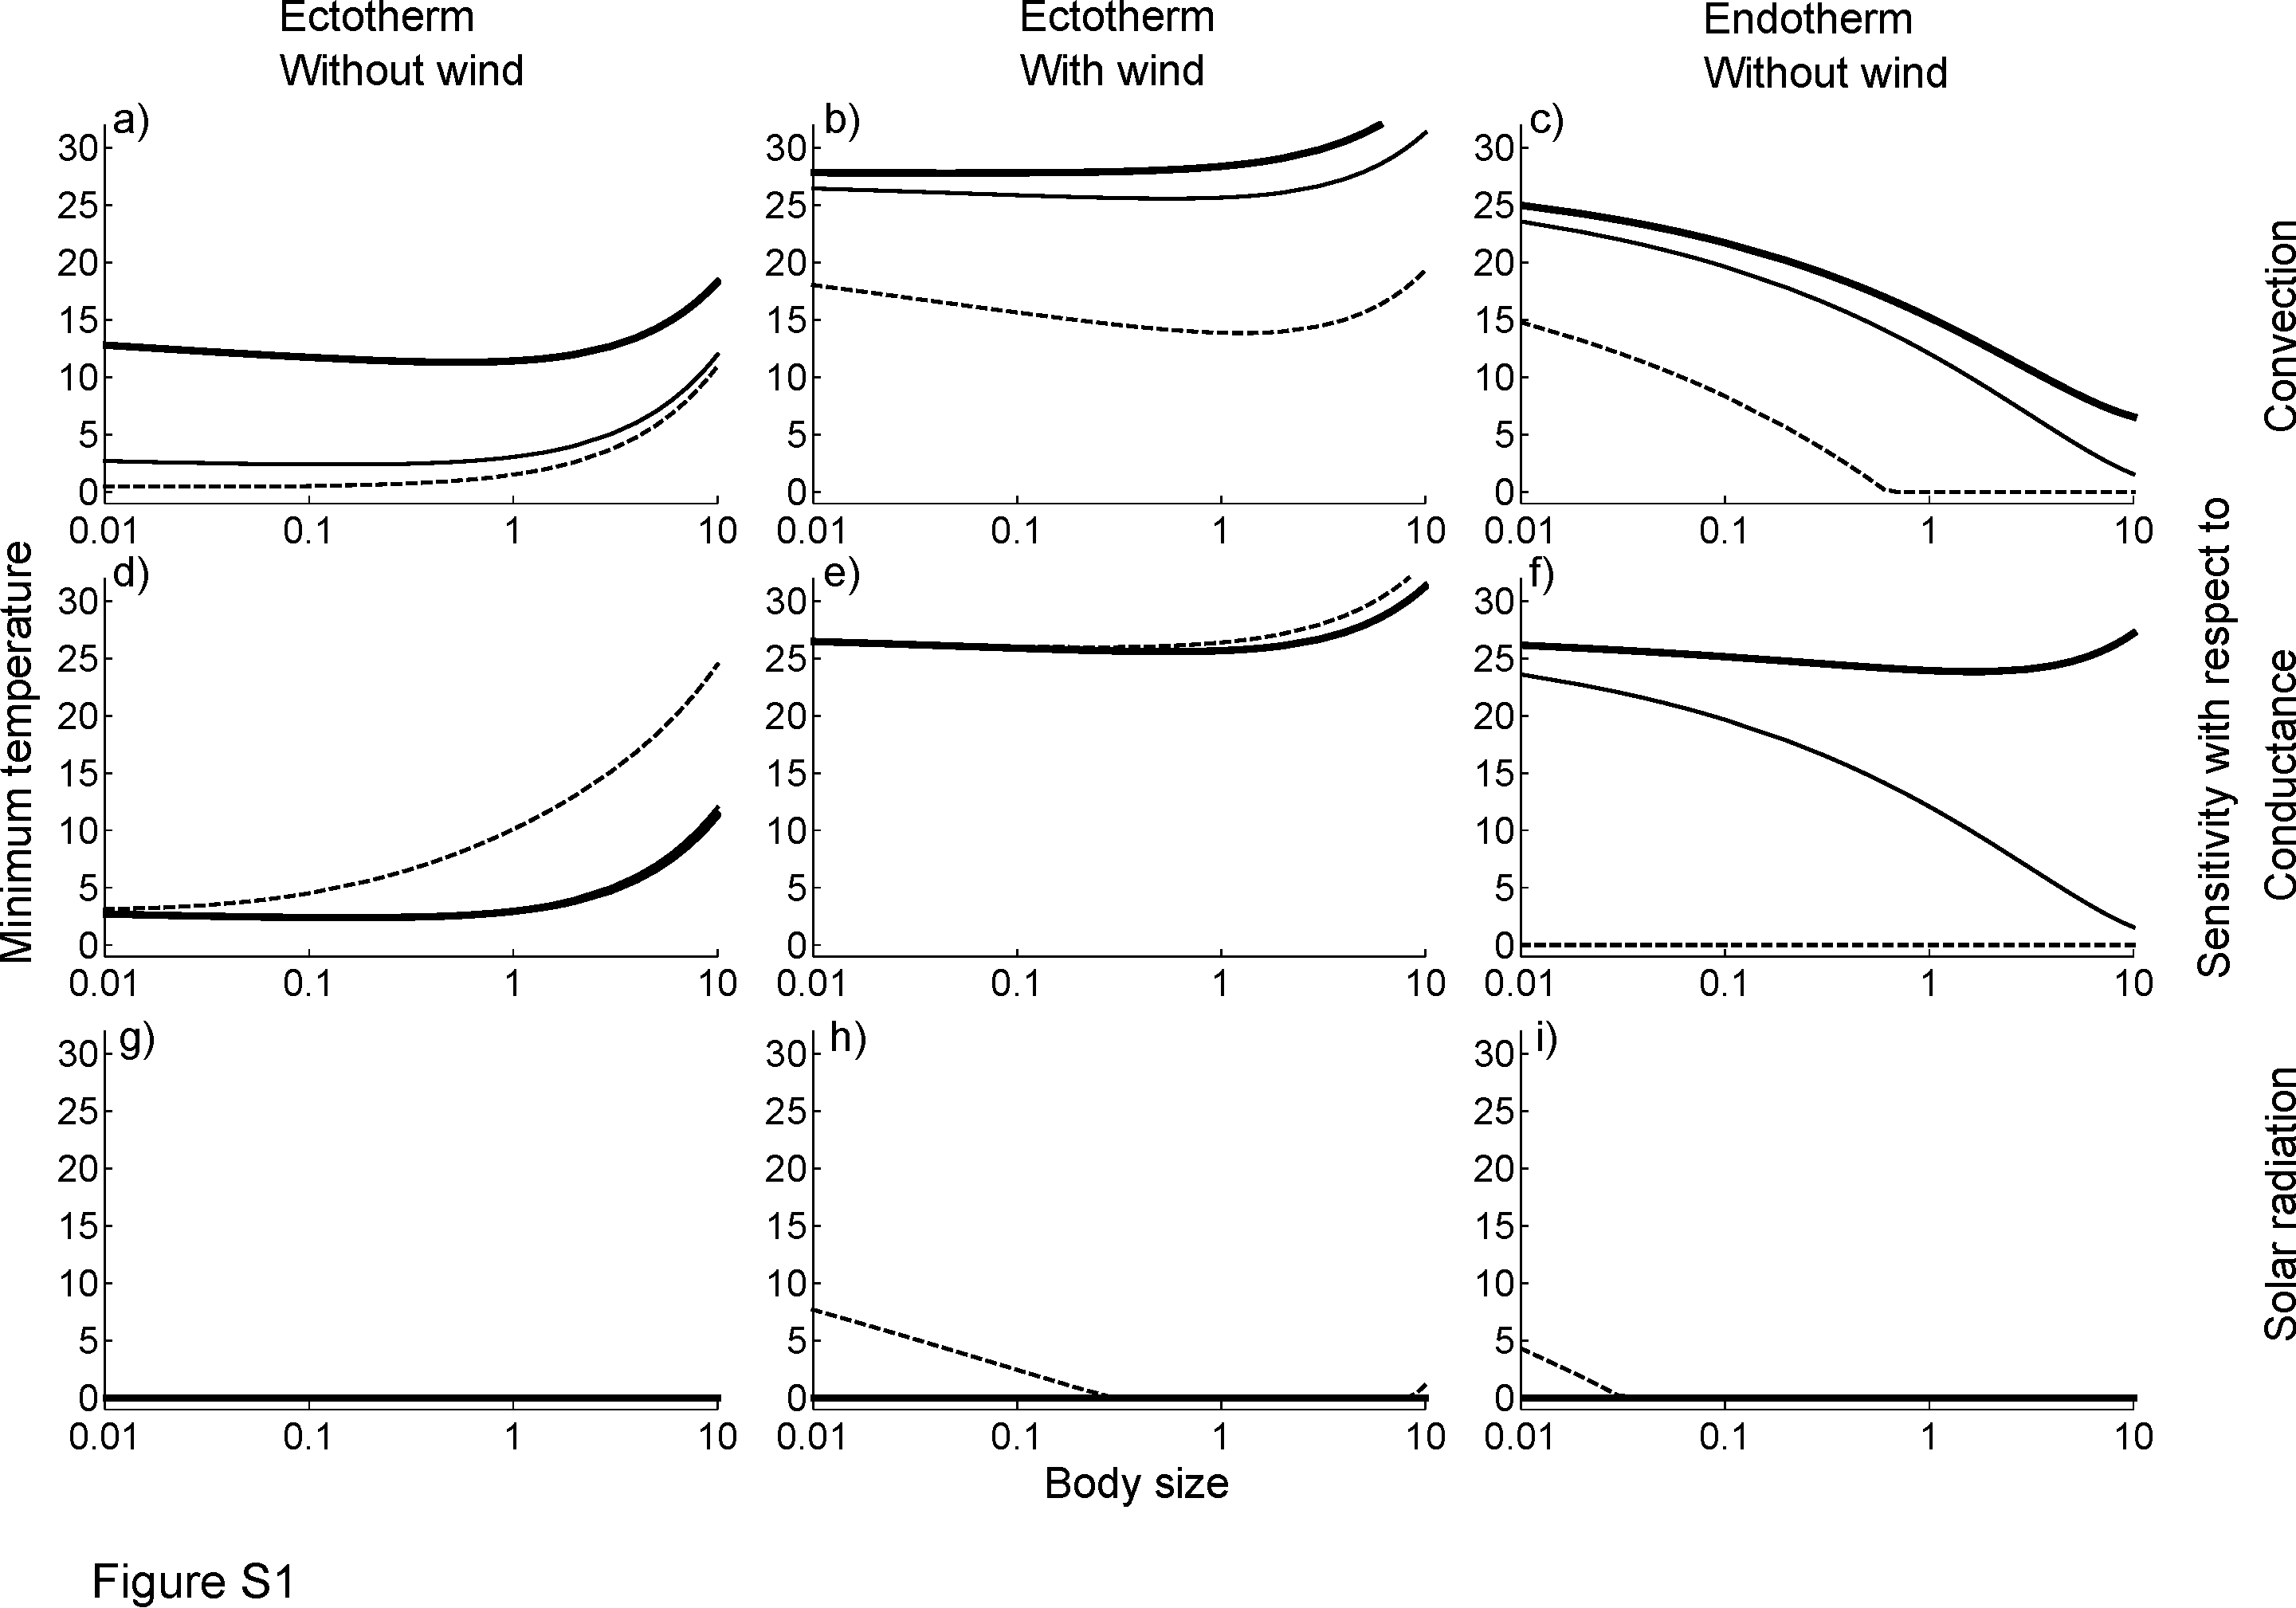
\includegraphics{figS1}}
	%\caption{Figure S1}
	\label{figS1}
%\end{center}
\end{figure*}


\begin{figure}
%\begin{center}
	\scalebox{0.85}{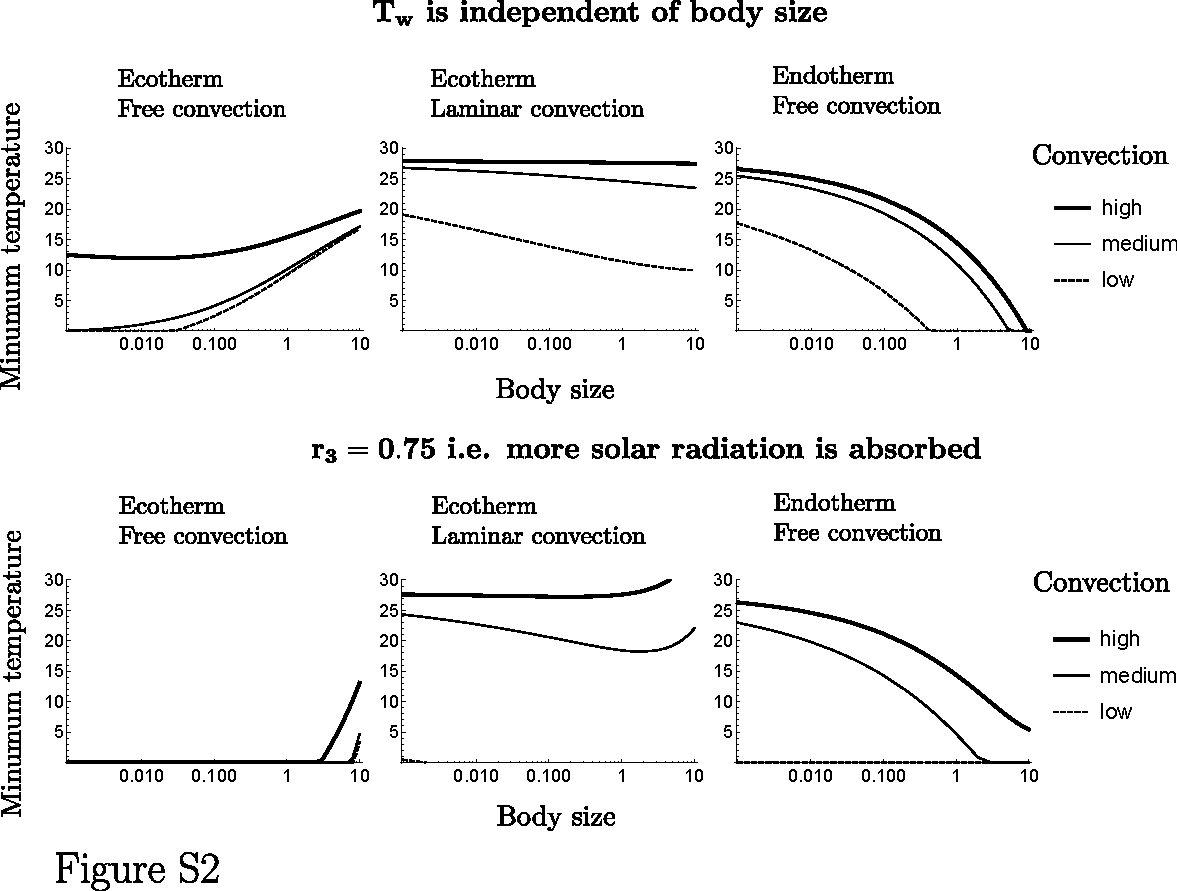
\includegraphics{figS2}}
	%\caption{Figure S2}
	\label{figS2}
%\end{center}
\end{figure}

\end{document}
